\documentclass[a4paper,11pt]{article}
\usepackage{indentfirst}
\usepackage[T1]{fontenc}
\usepackage[polish]{babel}
\usepackage[utf8]{inputenc}
\usepackage{lmodern}
\selectlanguage{polish}
\usepackage[top=2cm, bottom=2cm, left=1cm, right=1cm]{geometry}
\usepackage{lastpage}
\usepackage{fancyhdr}
\pagestyle{fancy}
\setlength\parindent{24pt}
\makeatletter
\newcommand{\linia}{\rule{\linewidth}{0.4mm}}
\renewcommand{\maketitle}{\begin{titlepage}
    \vspace*{2cm}
    \begin{center}\LARGE
    Politechnika Warszawska\\
    Wydział Elektryczny\\
    \end{center}
    \vspace{5cm}
    \noindent\linia
    \begin{center}
      \LARGE \textsc{\@title}
         \end{center}
     \linia
    \vspace{0.5cm}
    \begin{flushright}
    \begin{minipage}{5cm}
    \textit{Autor:}\\
    \normalsize \textsc{\@author} \par
    \end{minipage}
    \vspace{5cm}
     \end{flushright}
    \vspace*{\stretch{6}}
    \begin{center}
    \@date
    \end{center}
  \end{titlepage}
}
\makeatother
\author{Grzegorz Kopyt \\ Arkadiusz Michalak}
\title{Specyfikacja Funkcjonalna\\Projekt Zespołowy 2018/2019}
\usepackage{graphicx}

\fancyhf{}
\rfoot{\thepage{}/\pageref{LastPage}}

\begin{document}
\maketitle

\tableofcontents
\vspace{1cm}
\noindent\linia
\section{Wstęp teoretyczny}
Dokument ten dotyczy programu realizowanego w ramach ,,Projektu Zespołowego 2018/2019".

Głównym zadaniem jest analiza i podział terenu na optymalne części. Program na podstawie podanego konturu terenu oraz punktów kluczowych, znajdujących się na tym terenie, powinien podzielić go na optymalne części. Oznacza to, że każdy z powstałych obszarów powinien zawierać jeden punkt kluczowy, a granice powinny obejmować każde miejsce, z którego bliżej jest do danego punktu kluczowego niż do jakiegokolwiek innego z~punktów kluczowych.

Dodatkowo na całą mapę zostaną naniesione różne typy obiektów (między innymi domy z mieszkańcami), a~program powinien przygotować statystykę ilości obiektów oraz mieszkańców na danej części terenu.

Ważnym założeniem jest to, że pod danymi współrzędnymi może znajdować się tylko jeden punkt kluczowy lub obiekt.

Pozostałe funkcje programu zostały opisane w sekcji ,,Wymagania funkcjonalne".

\noindent\linia
\section{Wymagania funkcjonalne}

Program powinien spełniać podane wymagania funkcjonalne:
\begin{itemize}
\item podanie danych z pliku:
\begin{itemize}
\item podanie konturu terenu,
\item podanie rozmieszczeniem punktów kluczowych,
\item podawanie obiektów i definiowanie ich typów.
\end{itemize}
\item analiza terenu:
\begin{itemize}
\item podzielenie terenu na optymalne obszary,
\item wyświetlanie listy obiektów należących do danego obszaru,
\item wyświetlanie zbiorcze listy obiektów należących do danego obszaru,
\item wyświetlanie liczby mieszkańców danego obszaru.
\end{itemize}
\item wizualizacja:
\begin{itemize}
\item narysowanie granic optymalnych obszarów,
\item naniesienie na wczytany teren obiektów.
\end{itemize}
\item modyfikacja po wprowadzeniu danych z pliku:
\begin{itemize}
\item dodawanie i usuwanie elementów konturu terenu,
\item dodawanie i usuwanie punktów kluczowych,
\item nakładanie grafiki pod wyznaczone kontury.
\end{itemize}
\end{itemize}

Plik wejściowy powinien być zgodny z podanym wzorem:

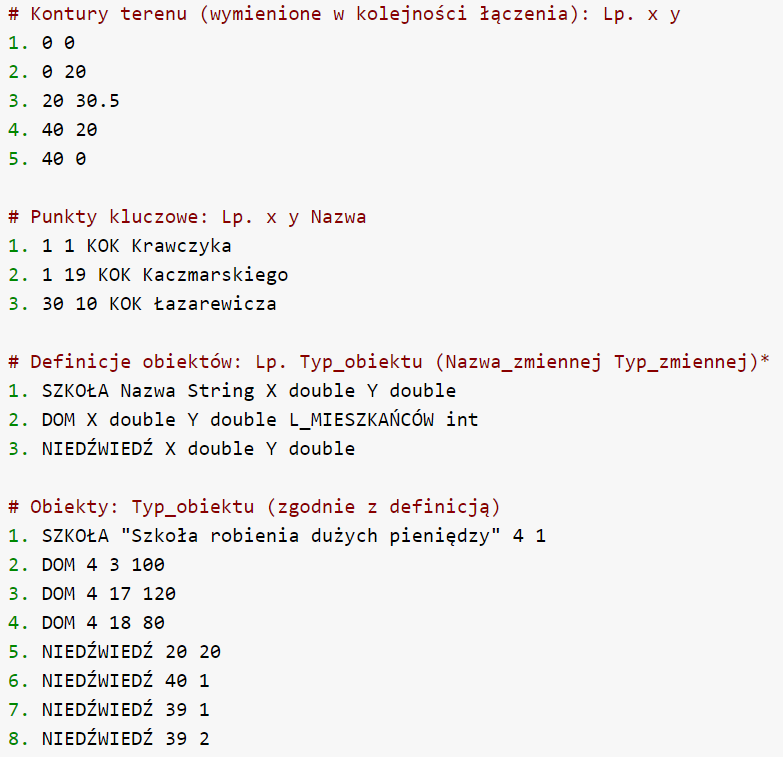
\includegraphics[scale=0.70]{ExampleInputFile}

Uwagi:
\begin{itemize}
\item kolejne sekcje pliku powinny być oddzielane znakiem \textit{\#};
\item obsługiwane typy możliwe do użycia przy definicji nowych typów to: string, int, double;
\item wartości zmiennych typu string powinny być podane w cudzysłowie;
\item nazwy obiektów powinny być bez spacji i zawierać do 40 znaków;
\item podane punkty kluczowe i obiekty muszą znajdować się wewnątrz podanego konturu terenu lub na jego krawędzi;
\item jeśli podany kontur będzie otwarty, ostatni jego punkt zostanie połączony z pierwszym;
\item podany kontur musi być figurą wypukłą;
\item krawędzie konturu terenu nie mogą się przecinać;
\item muszą zostać podane obiekty \textit{DOM}, \textit{NIEDŹWIEDŹ}, \textit{SZKOŁA} wraz z ich definicjami, takimi jak w pliku przykładowym;

\end{itemize}
\noindent\linia
\section{Obsługa}
\begin{itemize}
\item
\end{itemize}

\noindent\linia
\section{Komunikaty o błędach}
\begin{itemize}
\item
\end{itemize}

\noindent\linia
\section{Testy akceptacyjne}
\begin{itemize}
\item
\end{itemize}
\noindent\linia

\end{document}



